\subsection*{DESEMPENHO DO MODELO}
Resultados da Validação Cruzada
O desempenho do modelo foi avaliado utilizando validação cruzada (K-Fold Cross Validation) com 10 folds. A seguir estão os resultados de acurácia de validação para cada fold:

\begin{figure}[!h]
    \centering
    \caption{Resultado da Acurária ao longo dos treinamentos}
    \label{Gráfico 3}
    \includegraphics[width=0.9\linewidth]{Illustrations/tabela Acurácia.png}
\end{figure}

Análise da Acurácia Média A acurácia média de validação obtida ao longo dos 10 folds foi de 84.5\%, indicando um bom desempenho do modelo na tarefa de classificação. Esta métrica reflete a capacidade do modelo de generalizar bem para novos dados. 7 Variabilidade entre os Folds Houve alguma variação nos resultados de acurácia entre os diferentes folds, com um mínimo de 77.5\% e um máximo de 92.5\%.

\begin{figure}[!h]
    \centering
    \caption{Evolução da acurácia ao longo dos treinamentos}
    \label{Gráfico 3}
    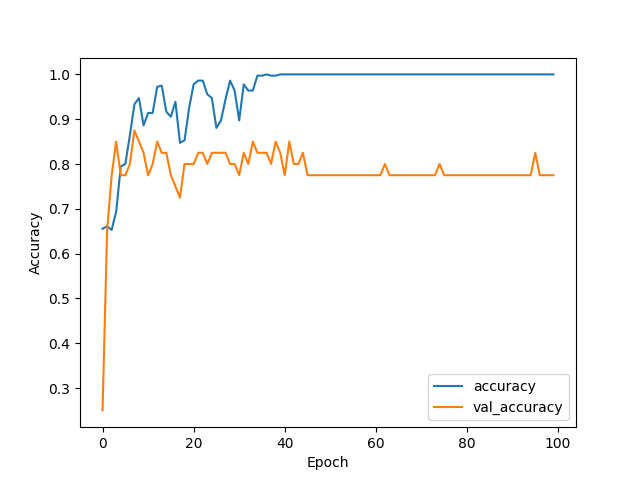
\includegraphics[width=0.7\linewidth]{Illustrations/Figure_1.png}
    \SourceOrNote{Autoria Própria (2025)}
\end{figure}

Esta variabilidade é esperada devido a diferenças na distribuição dos dados em cada fold e sugere que, enquanto o modelo performa consistentemente bem, há espaço para melhorias na generalização.Figura 3 O modelo foi treinado por 100 épocas com um batch size de 32, usando o otimizador Adam e a função de perda sparse categorical crossentropy. Este número de épocas foi suficiente para permitir ao modelo aprender as características dos dados sem sobreajustar aos dados de treinamento. A função de ativação ReLU nas camadas densas e softmax na camada de saída ajudaram a capturar relações não-lineares e a classificar corretamente as imagens.